\documentclass[border=8pt,tikz]{standalone}
\usepackage{tikz}
% Shared TikZ style for Chapter 5 diagrams.
% Inputted by every standalone diagram file.

\usetikzlibrary{
  arrows.meta,
  positioning,
  shapes.geometric,
  shapes.symbols,
  shapes.multipart,
  shapes.misc,
  fit,
  calc,
  backgrounds,
  decorations.pathmorphing,
  decorations.pathreplacing,
  patterns,
  shadows.blur,
}

% ─── Colour palette ──────────────────────────────────────────────
\definecolor{strixBlue}{HTML}{3B7DD8}     % data sources / inputs
\definecolor{strixGreen}{HTML}{22A699}    % processing / workers
\definecolor{strixOrange}{HTML}{E08036}   % storage
\definecolor{strixRed}{HTML}{E04B4B}      % attacker / external threat
\definecolor{strixPurple}{HTML}{6B5DD3}   % frontend / UI
\definecolor{strixGold}{HTML}{F2BE22}     % models / ML
\definecolor{strixGrey}{HTML}{6E7681}     % neutral / labels
\definecolor{strixDark}{HTML}{1F2933}     % titles / borders

% ─── Common node styles ──────────────────────────────────────────
\tikzset{
  >={Latex[width=2mm,length=2.5mm]},
  font=\sffamily\small,
  every node/.style={align=center},
  comp/.style={
    rectangle, rounded corners=2pt, draw=#1, fill=#1!10, very thick,
    text=strixDark, minimum width=22mm, minimum height=8mm,
    inner sep=4pt,
  },
  comp/.default=strixGreen,
  store/.style={
    cylinder, shape border rotate=90, aspect=0.3, draw=strixOrange,
    fill=strixOrange!12, very thick, text=strixDark,
    minimum width=18mm, minimum height=10mm, inner sep=2pt,
  },
  stream/.style={
    rectangle, rounded corners=2pt, draw=strixOrange,
    fill=strixOrange!8, dashed, thick, text=strixDark,
    minimum width=22mm, minimum height=7mm, inner sep=3pt,
    font=\ttfamily\scriptsize,
  },
  source/.style={comp=strixBlue},
  worker/.style={comp=strixGreen},
  model/.style={comp=strixGold},
  ui/.style={comp=strixPurple},
  ext/.style={comp=strixRed},
  title/.style={font=\sffamily\bfseries, text=strixDark},
  edge/.style={->, thick, draw=strixGrey, font=\sffamily\scriptsize\itshape},
  edgeStrong/.style={->, very thick, draw=strixDark, font=\sffamily\scriptsize\bfseries},
  group/.style={
    rectangle, rounded corners=4pt, draw=strixGrey, dashed, thick,
    inner sep=6pt, fill=strixGrey!4,
  },
  badge/.style={
    rectangle, rounded corners=1pt, fill=#1, text=white,
    font=\sffamily\scriptsize\bfseries, inner sep=2pt,
  },
  badge/.default=strixDark,
  port/.style={
    rectangle, rounded corners=1pt, draw=strixDark, fill=strixGrey!8,
    font=\ttfamily\scriptsize, minimum width=14mm, inner sep=2pt,
  },
}


\begin{document}
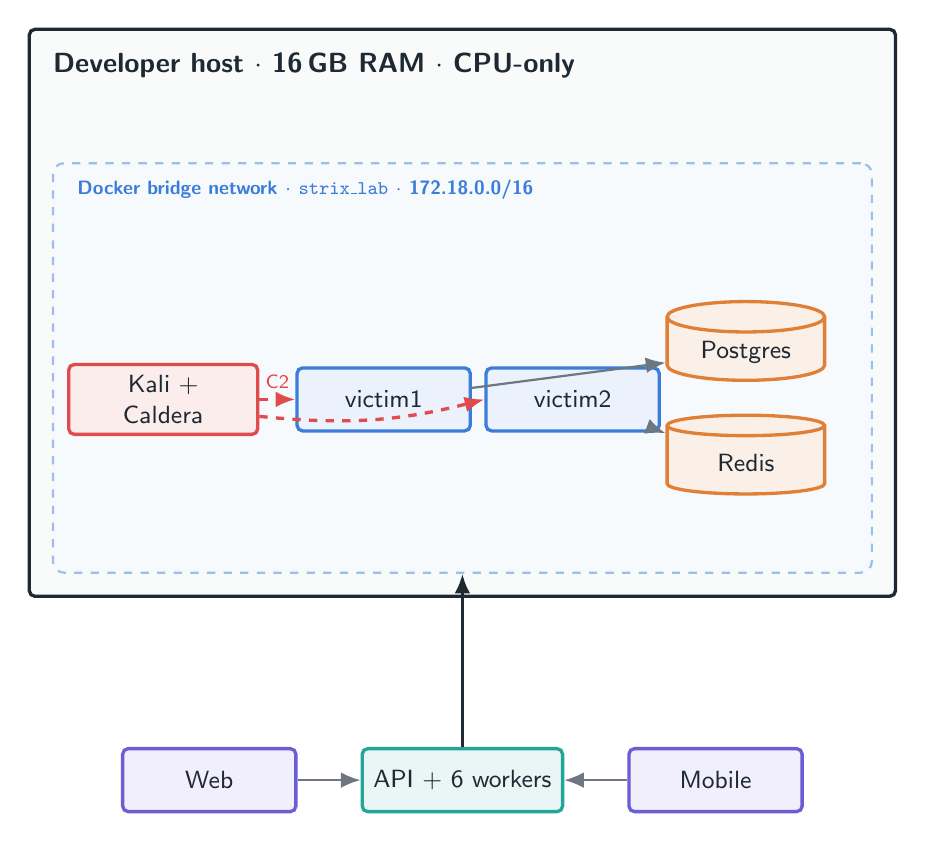
\begin{tikzpicture}[node distance=8mm]

% Developer host
\node[comp=strixDark, minimum width=110mm, minimum height=72mm,
      draw=strixDark, fill=strixGrey!4]
  (host) at (0,0) {};
\node[title, anchor=north west] at ([xshift=2mm,yshift=-2mm]host.north west)
  {Developer host \(\cdot\) 16\,GB RAM \(\cdot\) CPU-only};

% Docker bridge network
\node[group, minimum width=104mm, minimum height=52mm,
      fill=strixBlue!4, draw=strixBlue!50]
  (bridge) at (0,-7mm) {};
\node[title, font=\sffamily\bfseries\scriptsize, anchor=north west, text=strixBlue]
  at ([xshift=2mm,yshift=-1mm]bridge.north west)
  {Docker bridge network \(\cdot\) \texttt{strix\_lab} \(\cdot\) 172.18.0.0/16};

% Containers
\node[ext, minimum width=24mm]
  (attacker) at ([xshift=-38mm,yshift=-4mm]bridge.center) {Kali +\\Caldera};
\node[source, minimum width=22mm]
  (v1) at ([xshift=-10mm,yshift=-4mm]bridge.center) {victim1};
\node[source, minimum width=22mm]
  (v2) at ([xshift=14mm,yshift=-4mm]bridge.center) {victim2};
\node[store, minimum width=20mm]
  (pg) at ([xshift=36mm,yshift=2mm]bridge.center) {Postgres};
\node[store, minimum width=20mm]
  (rd) at ([xshift=36mm,yshift=-12mm]bridge.center) {Redis};

\node[worker, minimum width=22mm, anchor=north]
  (api) at ([yshift=-22mm]bridge.south) {API + 6 workers};
\node[ui, minimum width=22mm, left=8mm of api] (web) {Web};
\node[ui, minimum width=22mm, right=8mm of api] (mob) {Mobile};

\draw[edgeStrong, dashed, draw=strixRed]
  (attacker.east) -- (v1.west) node[midway,above,font=\sffamily\scriptsize, text=strixRed] {C2};
\draw[edgeStrong, dashed, draw=strixRed]
  (attacker) to[bend right=10] (v2.west);
\draw[edge] (v1) -- (pg);
\draw[edge] (v2) -- (rd);
\draw[edgeStrong] (api) -- (bridge.south);
\draw[edge] (web) -- (api);
\draw[edge] (mob) -- (api);

\end{tikzpicture}
\end{document}
